\documentclass[sigconf]{acmart}

\usepackage{hyperref}

%\usepackage{endfloat}
%\renewcommand{\efloatseparator}{\mbox{}} % no new page between figures

\usepackage{booktabs} % For formal tables

\settopmatter{printacmref=false} % Removes citation information below abstract
\renewcommand\footnotetextcopyrightpermission[1]{} % removes footnote with conference information in first column
\pagestyle{plain} % removes running headers


\begin{document}
	
	\title{Predicting Housing Prices - Kaggle Competition}	
	
	\author{Murali Cheruvu, Anand Sriramulu}
	\orcid{xxxx-xxxx-xxxx}
	\affiliation{%
		\institution{Indiana University}
		\streetaddress{3209 E 10th St}
		\city{Bloomington} 
		\state{Indiana} 
		\postcode{47408}
	}
	\email{mcheruvu@iu.edu, asriram@iu.edu}
	
	% The default list of authors is too long for headers}
	\renewcommand{\shortauthors}{M. Cheruvu, A Sriramulu}
	
	
	\begin{abstract}
		
		Apply exploratory data analysis and implement various advanced supervised machine learning algorithms to predict neighborhood housing sale prices found in the sample test dataset. Compare the predicted models and results from these advanced supervised algorithms. Apply ensembled model to achieve better predictions, hence get good score in kaggle competition.
		
	\end{abstract}
	
	\keywords{i523, hid306, Supervised Learning Algorithms, Exploratory Data Analysis, Kaggle}
	
	\maketitle
	
	\section{Introduction} % The \section*{} command stops section numbering
	
	Part of the kaggle competition, two sample data sets are given with 80 attributes (variables) describing various aspects of the residential homes in Ames and Iowa cities. Training dataset contains sale price of the homes, and using this training data set, how accurately we can predict Sale Prices of the homes in the test dataset using preprocessing and thorough data analysis. Many developers used advanced learning algorithms - XGBoost, Lasso and Neural Network, to predict the sale prices in the kaggle competition and achieved better kaggle scores. Kaggle score is a measure to indicate accuracy and the quality of the algorithm. We have applied various exploratory analysis techniques and engineer the features before applying a few advanced supervised learning algorithms.   
	
	\section{Exploratory Data Analysis} 
	
	There are 1460 rows in the training data set and 1459 rows in the test dataset. Out of the 80 variables, 23 are nominal, 23 are ordinal, 14 are discrete, and 20 are continuous. We have combined training and testing datasets for easier analysis. We excluded Id attribute as it does not add value in the modeling. We also removed Sale Price, the target variable, from the training dataset. All attribute details are given in the appendix section as a reference.
	\subsection{Handling Missing Values}
	
	First part of the analysis, we have checked for the missing values in the dataset. we have also identified that there are 6 variables having most of the missing data. All the missing values for the numeric variables are analyzed further to decide whether to delete the instances of the data with missing values or fill them using meaningful data such as median of the corresponding variable.
	
	\begin{verbatim}
	
	# python code - check for null values
	train = pd.read_csv("../data/train.csv")
	test = pd.read_csv("../data/test.csv")
	
	
	#combine the data sets
	alldata = train.append(test)	
	na = alldata.isnull().sum()
	.sort_values(ascending=False)
	\end{verbatim}
	
	\begin{figure}[H]
		\centering
		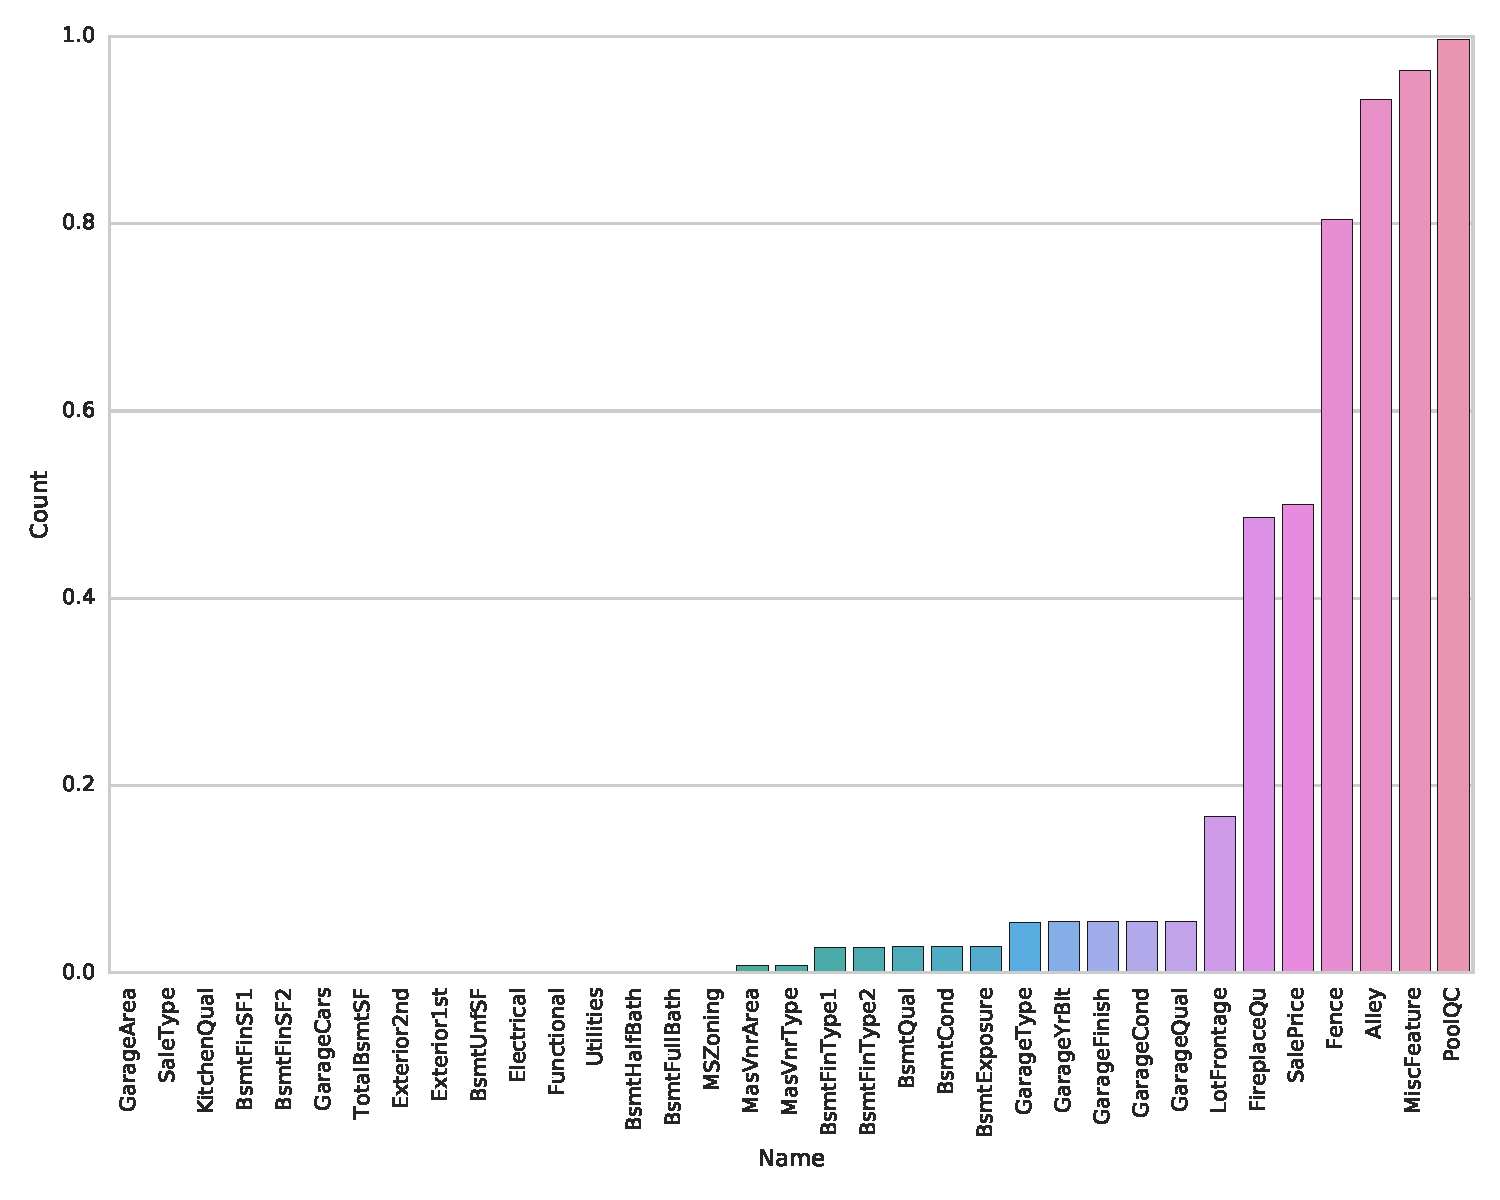
\includegraphics[width=0.9\columnwidth]{images/missing_values}	
		\caption{Variables with Missing Values} \label{fig:missing_values} 
	\end{figure}
	
	\subsection{Analyze Numerical Variables}
	There are 37 numeric variables after excluding the {\em Id} variable. We have analyzed the numeric variables for data patterns such as skewed data and range of the possible values. {\em  over all quality}, {\em ground living area}, {\em garage cars} and {\em garage area} graphs are included as samples.
	\begin{verbatim}
	# python code - analyze numeric variables
	numerical_features = [f for f in train.columns 
	if train.dtypes[f] != 'object']
	
	nd = pd.melt(train, value_vars = numerical_features)	
	plt.figure(figsize = (5,3))
	plot = sns.FacetGrid (nd, col='variable', col_wrap=4,
	sharex=False, sharey = False)
	plot = plot.map(sns.distplot, 'value')				
	\end{verbatim}
	
	\begin{figure}[H]
		\centering
		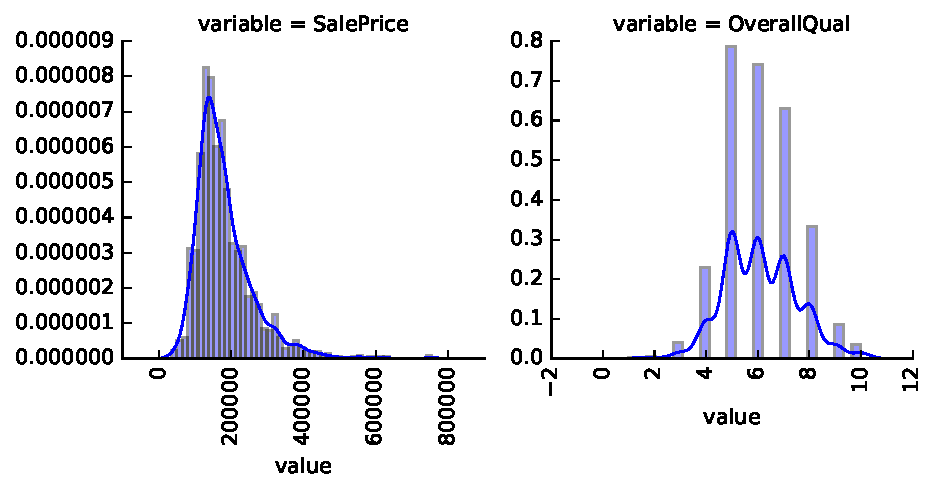
\includegraphics[width=0.75\columnwidth]{images/num_features_1}			
	\end{figure}
	
	\begin{figure}[H]
		\centering
		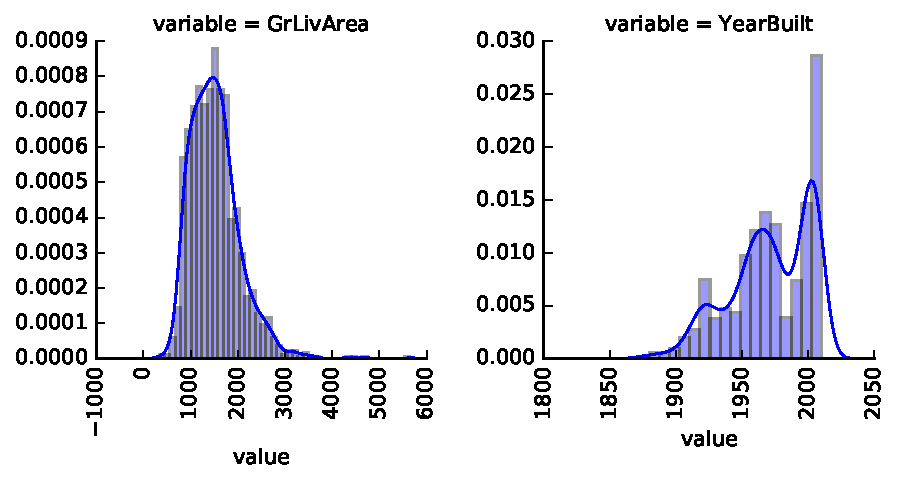
\includegraphics[width=0.75\columnwidth]{images/num_features_2}	
		\caption{Sample Numerical Variables} \label{fig:num_features_2} 
	\end{figure}
	
	\subsection{Analyze Categorical Variables}
	There are 43 categorical variables in the dataset. We have analyzed all categorical variables and found the ways to fill the missing values and also the way we need to convert them into numerical variables. Later in the feature engineering section, we will go through the details. {\em neighborhood} and {\em sale type} graphs are included as samples.
	\begin{verbatim}
	
	# python code - analyze numeric variables
	cat_features = [f for f in train.columns 
	if train.dtypes[f] == 'object']
	print(cat_features)
	
	def barplot(x,y,**kwargs):
	sns.barplot(x=x,y=y)
	x = plt.xticks(rotation=90)
	
	plt.figure(figsize = (5,3))
	
	p = pd.melt(train, id_vars='SalePrice',
	value_vars=cat_features)
	
	g = sns.FacetGrid (p, col='variable', col_wrap=4, 
	sharex=False, sharey=False, size=5)
	
	g = g.map(barplot, 'value','SalePrice')				
	\end{verbatim}
	
	\begin{figure}[H]
		\centering
		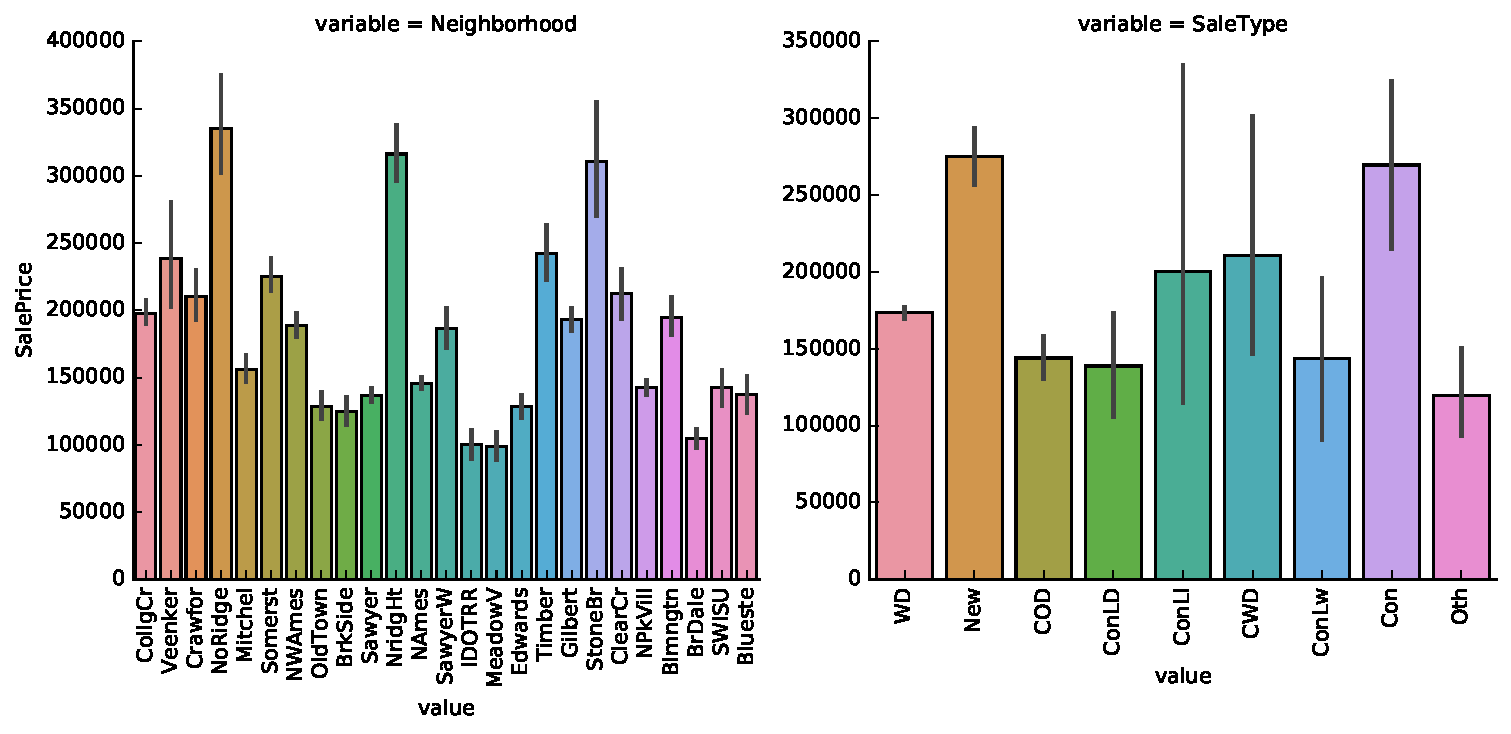
\includegraphics[width=1.0\columnwidth]{images/cat_features_1}	
		\caption{Sample Category Variables} \label{fig:cat_features_1} 
	\end{figure}
	
	\subsection{Analyze Correlations}		
	{\em Numpy} package offers correlations functionality to analyze the variables that highly positively or negatively correlated with {\em sale price} and with the other variables. We can  visualize a few pair-wise correlation graphs with sale price for detailed analysis. From the correlation-plot we can list the top 10 features those are strongly correlated with the target variable - {\em sale price}.
	
	\begin{verbatim}
	
	# python code 
	corr = alldata[numerical_features].corr()	
	mask = np.zeros_like(corr)
	mask[np.triu_indices_from(mask)] = True	
	plt.figure(figsize = (15,8))	
	sns_plot = sns.heatmap(corr, cmap="YlGnBu", 
	linewidths=.5,  mask=mask, vmax=.3)	
	\end{verbatim}
	
	\begin{figure}[H]
		\centering
		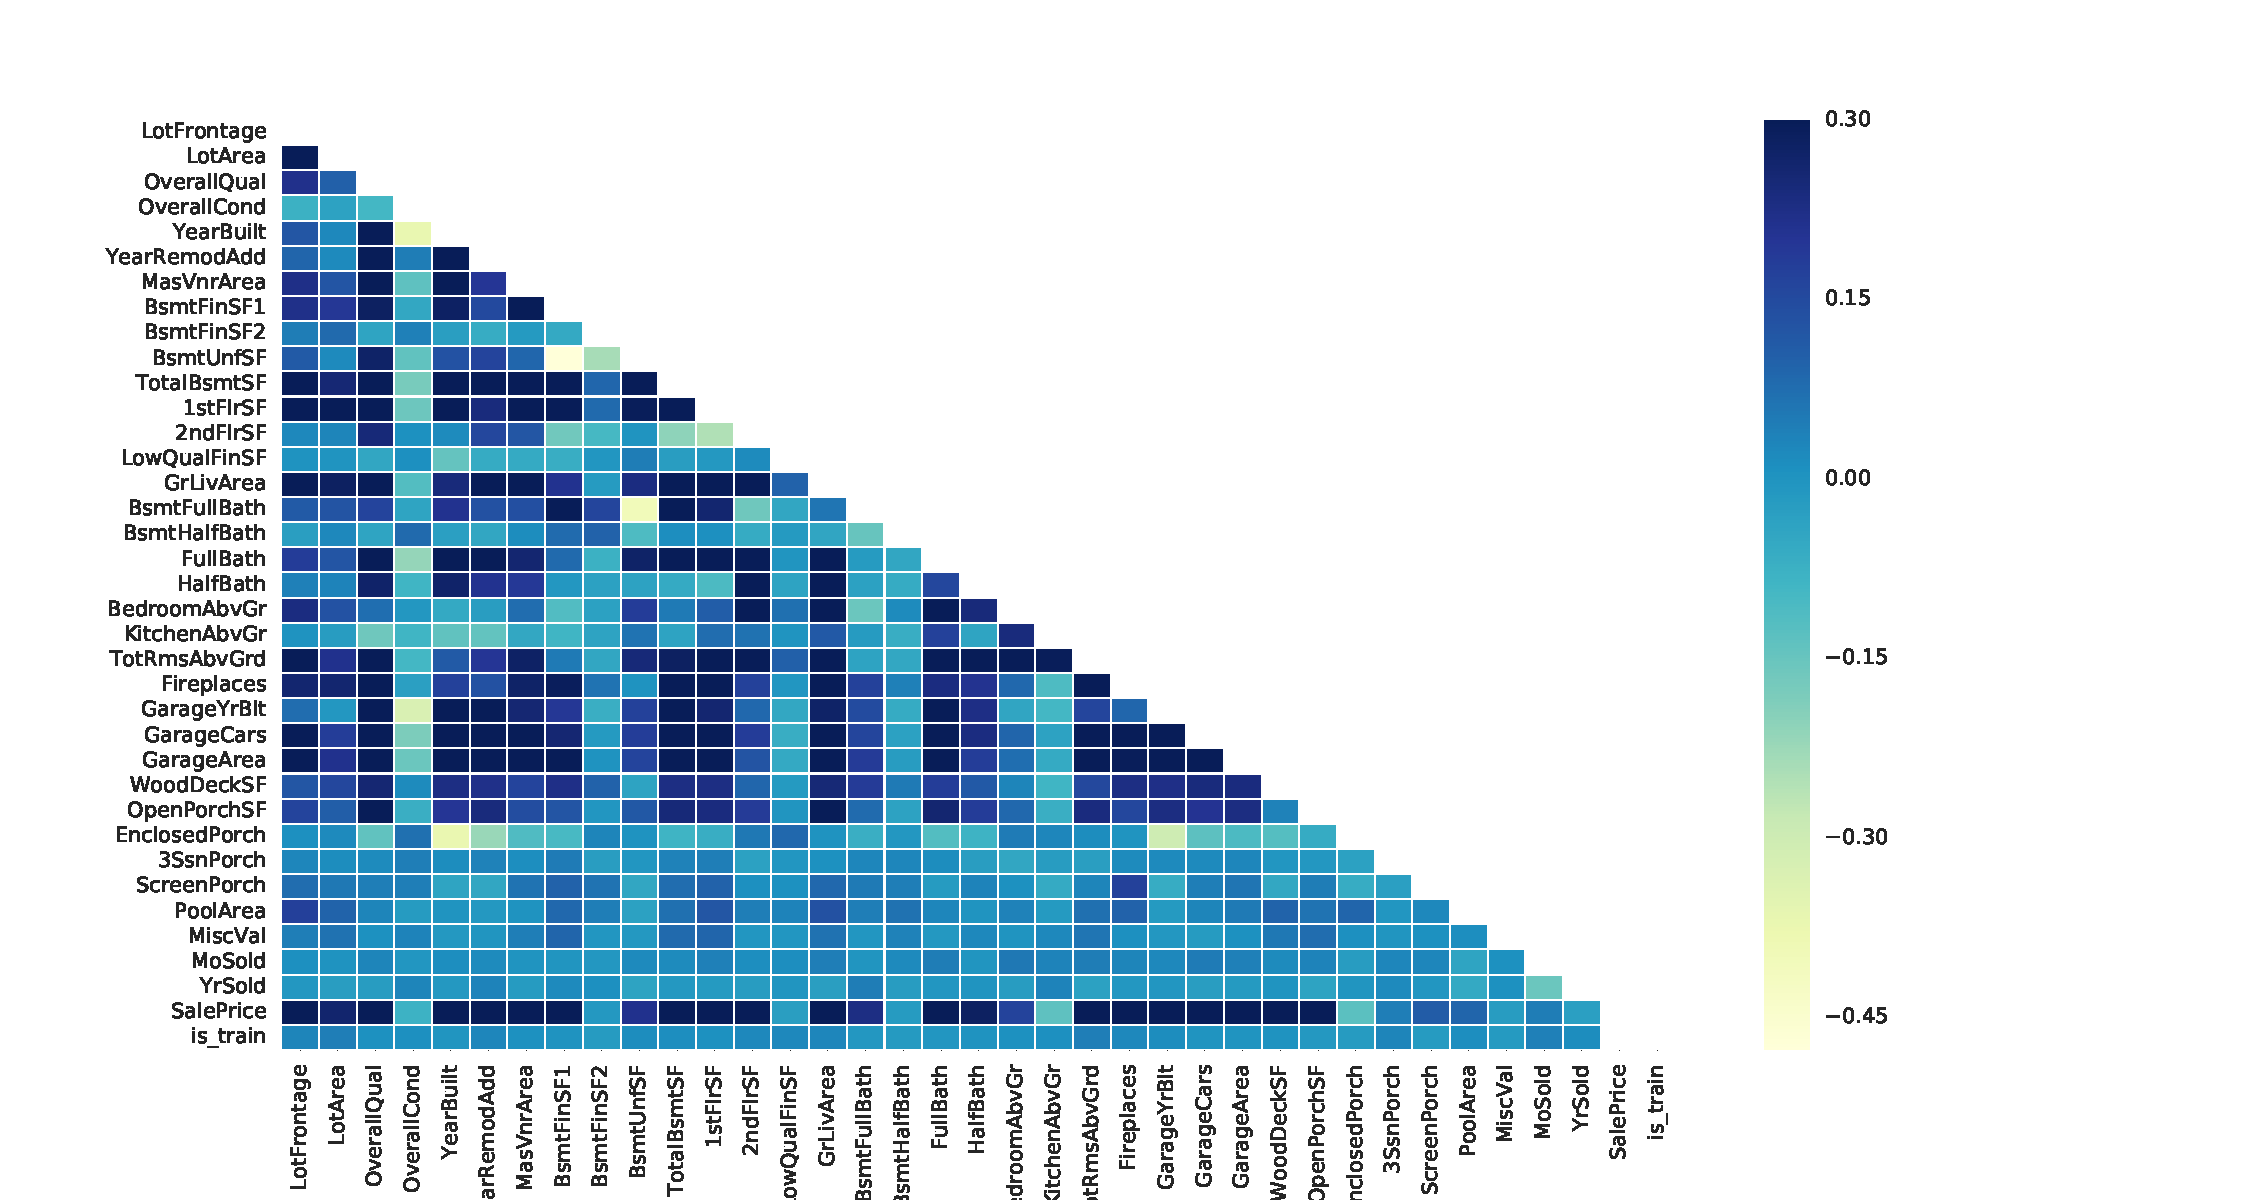
\includegraphics[width=1.2\columnwidth]{images/correlations}	
		\caption{Correlations} \label{fig:correlations} 
	\end{figure}
	
	\begin{figure}[H]
		\centering
		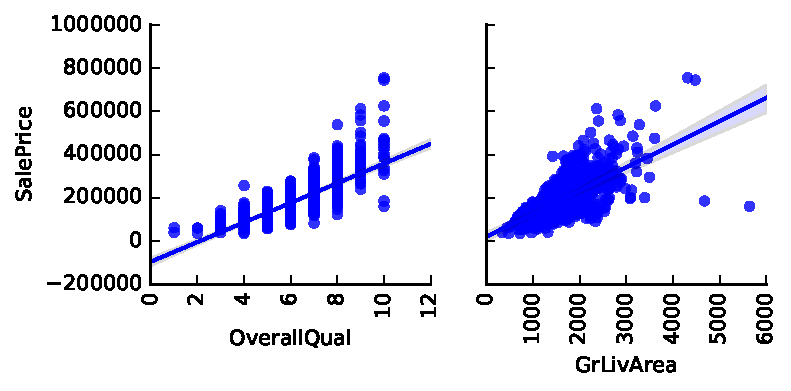
\includegraphics[width=0.9\columnwidth]{images/pair_wise_correlations_1}	
	\end{figure}
	
	\begin{figure}[H]
		\centering
		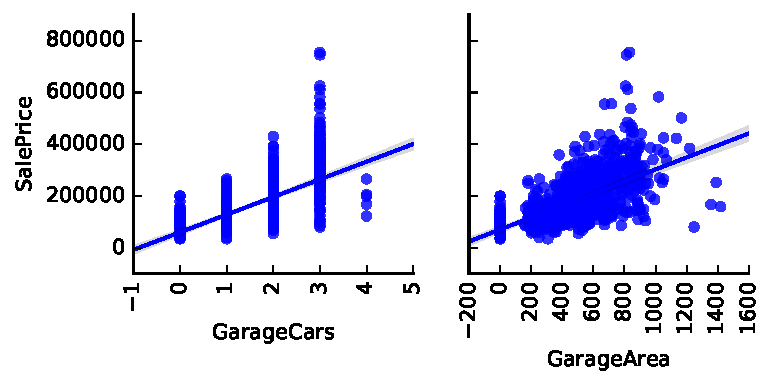
\includegraphics[width=0.9\columnwidth]{images/pair_wise_correlations_2}	
		\caption{Pair-wise Correlations with Sale Price} \label{fig:pair_wise_correlations_2} 
	\end{figure}
	
	\begin{enumerate}
		\item OverallQual: Overall material and finish quality
		\item GrLivArea: Above ground living area square feet
		\item GarageCars: Size of garage in car capacity
		\item GarageArea: Size of garage in square feet
		\item TotalBsmtSF: Total square feet of basement area
		\item 1stFlrSF: First Floor square feet
		\item FullBath: Full bathrooms above grade
		\item TotRmsAbvGrd: Total rooms above ground
		\item YearBuilt: Original construction date
		\item GarageYrBlt: Garage built year		
	\end{enumerate}
	
	\subsection{Skewed Data Analysis}
	From the numerical analysis, we have identified that there are a few numerical variables need further analysis to identify the skewed data. We did not find any key variables those have skewed more than 75\%. However, we wanted to replace the {\em sale price} with corresponding logarithmic value for the predictive models and later convert it back to the exponential value before submitting to the kaggle competition. 
	
	\subsection{Outlier Analysis}
	
	Continuing with exploratory analysis, We have analyzed the outliers using {\em Cook's distance} and then further analyzed two key variables - {\em ground live area} and {\em garage area} that are in high correlation with {\em sale price}. We have removed the outlier rows related to these two variables as they are only 8 rows impacting the training dataset.
	
	\begin{verbatim}
	
	# python code - outlier analysis
	import statsmodels.api as sm
	from statsmodels.formula.api import ols
	
	model = ols(formula = "SalePrice ~ 
	GrLivArea + GarageArea", data=train)
	fitted = model.fit()    	
	plot = sm.graphics.influence_plot(fitted, 
	criterion="cooks")		
	\end{verbatim}
	
	\begin{figure}[H]
		\centering
		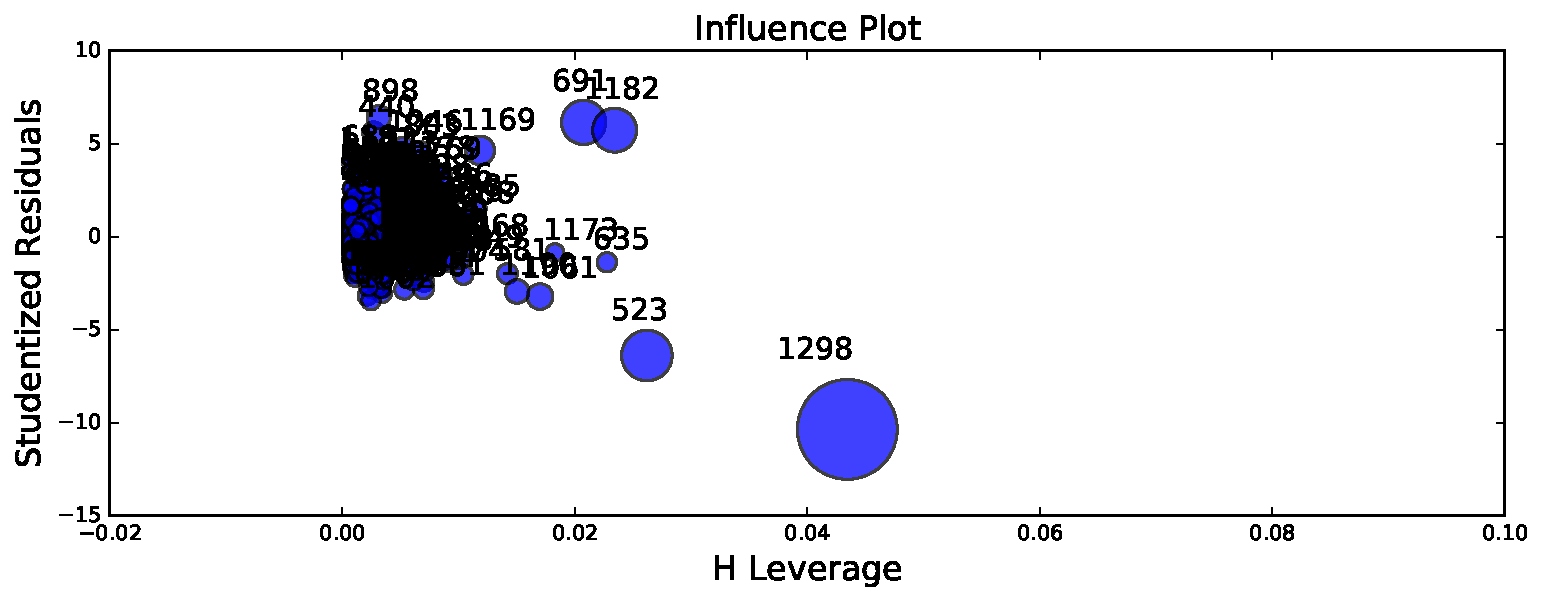
\includegraphics[width=.95\columnwidth]{images/outliers}	
		\caption{Outliers - Cook's distance} \label{fig:outliers} 
	\end{figure}
	
	\begin{verbatim}
	
	# python code - remove outlier rows
	# fix all extreme outliers based on outlier analysis
	# 8 rows will be deleted
	train = train[train.GrLivArea <= 4000]
	train = train[train.GarageArea <= 1200]
	\end{verbatim}
	
	\begin{figure}[H]
		\centering
		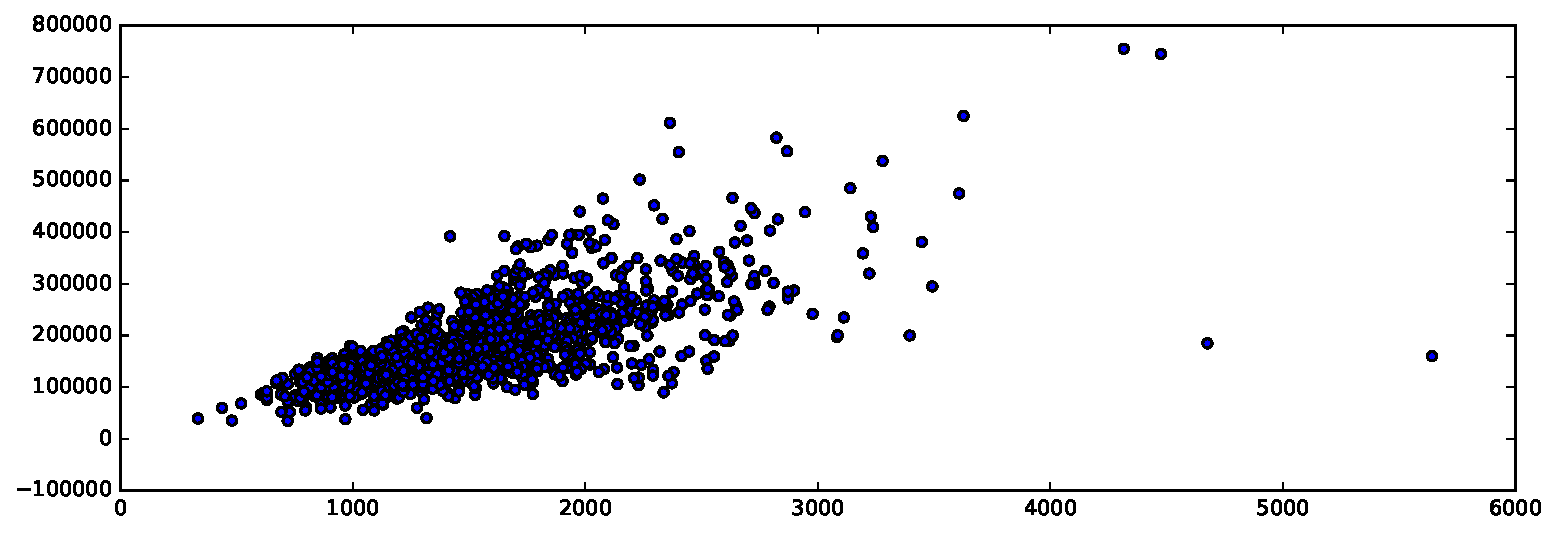
\includegraphics[width=.95\columnwidth]{images/gr_liv_area_outlier}	
		\caption{Outliers - Garage Live Area} \label{fig:gr_liv_area_outlier} 
	\end{figure}
	
	\begin{figure}[H]
		\centering
		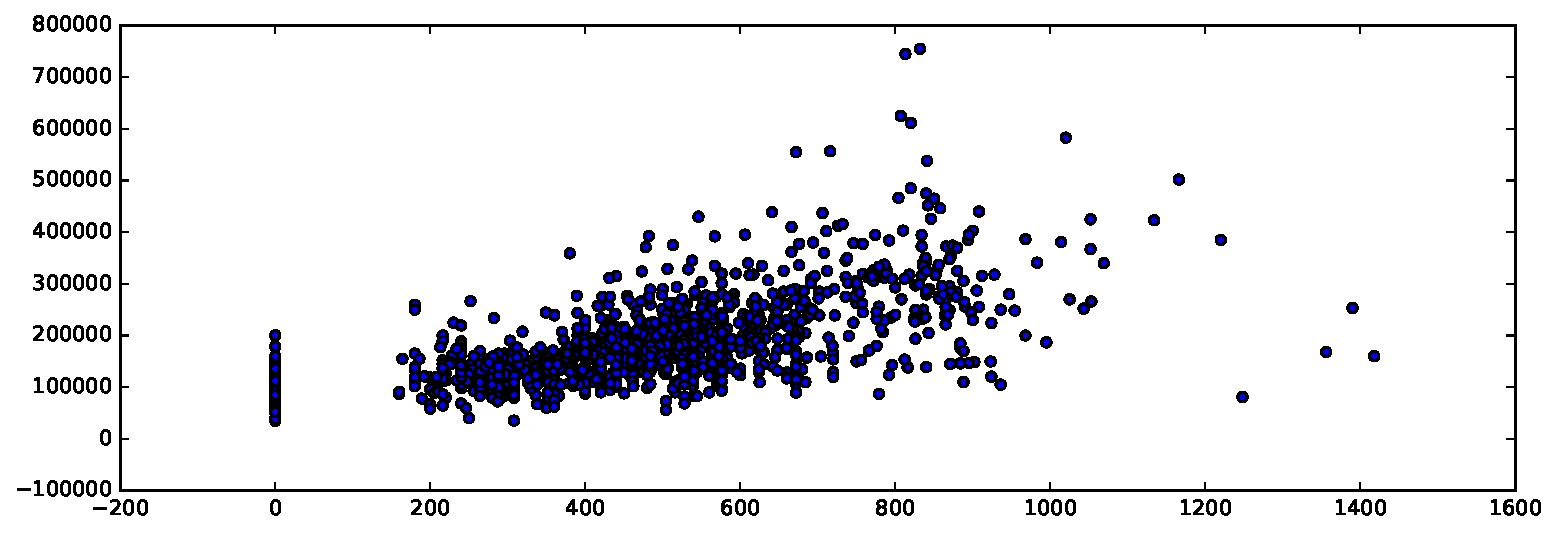
\includegraphics[width=.95\columnwidth]{images/garage_area_outlier}	
		\caption{Outliers - Garage Area} \label{fig:garage_area_outlier} 
	\end{figure}
	
	\subsection{Feature Engineering}
	
	Feature engineering is a technique to analyze all the variables those influence target variable for better predictions. Part of feature engineering, we may need to create new featues to make the data to be more expressive. One of the key intents, in analyzing categorical variables, is to convert them into numerical factors as most of the machine learning algorithms expect all the variables to be numeric for them to work more effectively. Some of the categorical variables are ordinal. we can use T-shirt sizes: small, medium and large as an example to explain an ordinal variable. When we convert this category variable into numeric encoding, we need to retain the fact that there is an implicit order within the values. Supposing we give ordinal encoding as - small = 1, medium = 2 and large = 3; we will satisfy the implicit order or weightage and that helps in modeling the system by elevating the importance of this implicit ordering in the values of the ordinal variable.
	
	There are a few other encoding techniques, such as one-hot, binary, polynomial and helmert to factorize categorical variables. We will use ordinal and one-hot encoding techniques for this data set. One-hot encoding converts the category variable into many binary vectors, one new numeric variable for each value in the category. Assume that we have a category variable called signal-light with three possible values: green, yellow and red. We will need to convert these values into numeric - green = 1, yellow = 2 and red = 3. When we apply one-hot encoding on this variable, basically we are creating three new categorical variables - signal-light-green, signal-light-yellow and signal-light-red along with the original variable - signal-light, each is pretty much a binary vector having 1s for all the corresponding values; otherwise 0s. With hot-encoding, we are basically increasing the dimensions in the model. After extensive feature engineering applied on the housing dataset, we have added {\em 228} new features (variables). Following are the python methods to factorize categorical variables and one-hot encoding techniques. 
	
	\begin{verbatim}
	
	# python code - factorize and one-hot
	def get_one_hot(df, col_name, fill_val):
	if fill_val is not None:
	df[col_name].fillna(fill_val, inplace=True)
	
	dummies = pd.get_dummies(df[col_name], prefix="_" + col_name)
	df = df.join(dummies)
	df = df.drop([col_name], axis=1)
	return df
	#end def
	
	from sklearn.preprocessing import LabelEncoder
	
	def factorize(df, column, fill_na=None):
	le = LabelEncoder()
	if fill_na is not None:
	df[column].fillna(fill_na, inplace=True)
	le.fit(df[column].unique())
	df[column] = le.transform(df[column])
	return df
	#end def
	\end{verbatim}
	
	\section{Algorithms and Methodology}
	
	Linear regression predicts the target variable using best possible straight line fit to the set predictor variables. The possible best fit is usually the one that minimizes the root mean squared error (RMSE) between the actual and predicted data points. However, with complex problem space such as the housing prices dataset, we have lots of variables relating to the target variable in a non-linear fashion. Trivial supervised learning algorithms will not be effective to provide accurate {\em sale price} predictions. To overcome this challenge, we have applied various advanced supervised learning algorithms, such as Support Vector Machine (SVM), Random Forest, Lasso, Ridge, XGBoost and Neural Network, to predict the test data housing prices.
	
	
	\subsection{Support Vector Machine (SVM) Algorithm}
	
	Support Vector Machine (SVM) algorithms can be used to solve classification and regression problems. SVM regression relies on kernel functions for modeling the data. SVM creates larger margins between categories of data so that they are linearly separable. SVM handles non-linearly separable data, mainly for regression problems, using kernel functions, such as polynomial, radial basis function (RBF) and sigmoid, to project the data onto a hyperplane. Following python code snippet is the implementation for {\em sale price} predictions of the housing test dataset.
	
	\begin{verbatim}
	
	# python code - SVM algorithm
	from sklearn.svm import SVR
	import matplotlib.pyplot as plt
	from sklearn.metrics import mean_squared_error
	
	train = pd.read_csv("train.csv")
	test = pd.read_csv("test.csv")
	target_vector = train["SalePrice"]
	
	_svm_algo = SVR(kernel = 'rbf', C=1e3, gamma=1e-8)	
	
	_svm_algo.fit(train, target_vector)    
	
	y_train = target_vector
	y_train_pred = _svm_algo.predict(train)
	
	#root mean squared error (RMSE)
	rmse_train = np.sqrt(rmse(y_train,y_train_pred))
	
	y_test_pred = _svm_algo.predict(test)
	
	\end{verbatim}
	
	
	\subsection{Random Forest Algorithm}
	
	Random Forest is an advanced machine learning algorithm for predictive analytics. Random Forest ensembles multiple decision trees to create an additive learning model from the sequence of base models created by each decision tree that worked on a sub-sample dataset. Random Forest models are suitable to handle tabular datasets with hundreds of numeric and categorical features. Along with missing values, non-linear relations between features and the target, will be handled well by random forest algorithms. With proper tuning of hyper-parameters of the random forest algorithm, it can perform well with decent accuracy in the predictions without overfitting the model. Unlike similar regression models, it does not offer feature coefficient information but it provides {\em feature ranking} functionality very nicely. Following are the random forest algorithm details for the {\em sale price} predictions implemented in python using {\em sklearn} package.
	
	\begin{verbatim}		
	# python code - random forest algorithm
	from sklearn.ensemble import RandomForestRegressor
	from sklearn.metrics import accuracy_score
	from sklearn.metrics import confusion_matrix
	from sklearn.metrics import mean_squared_error
	
	train = pd.read_csv("train.csv")
	test = pd.read_csv("test.csv")
	target_vector = train["SalePrice"]
	
	_algo = RandomForestRegressor(n_estimators=100, 
	oob_score=True, random_state=123456)
	
	model = _algo.fit(train, target_vector)  
	
	feat_imp = pd.Series(_algo.feature_importances_, 
	train.columns).sort_values(ascending=False)
	
	feat_imp[:10].plot(kind='bar', 
	title='Feature Ranmkingt')		
	y_train = target_vector
	y_train_pred = _algo.predict(train)
	
	#root mean squared error (RMSE)
	rmse_train = np.sqrt(rmse(y_train,y_train_pred))			
	y_test_pred = _algo.predict(test)		
	\end{verbatim}
	
	
	\begin{figure}[H]
		\centering
		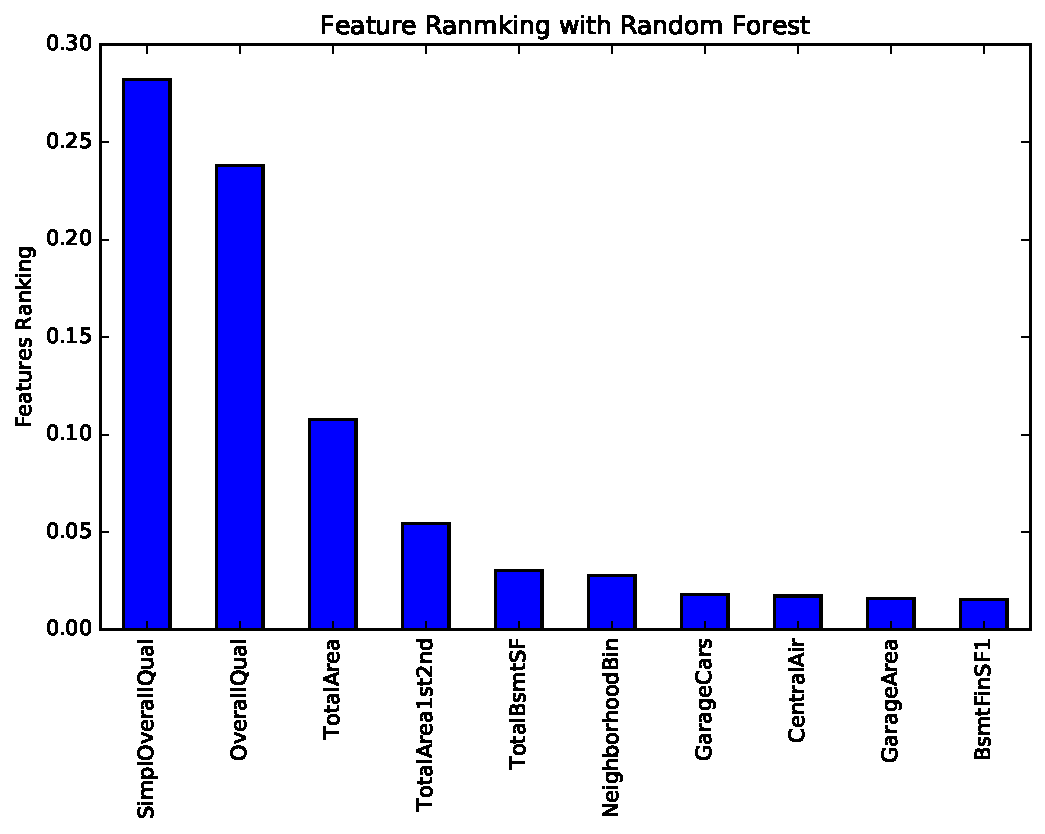
\includegraphics[width=0.85\columnwidth]{images/random_forest_feature_ranking}	
		\caption{Random Forest Feature Ranking} \label{fig:random_feature_ranking} 
	\end{figure}
	
	\subsection{Lasso Algorithm}
	
	
	
	\subsection{Ridge Algorithm}
	
	Ridge algorithm is very similar to lasso algorithm with the same goal. While lasso performs {\em L1 regularization}, ridge applies {\em L2 regularization} techniques in modeling the predictions. L1 regularization adds penalty to the variables equivalent to {\em absolute value of the magnitude} of the coefficients, where as L2 adds the penalty equivalent to {\em square of the magnitude} of the variable coefficients. Following is the python implementation of the ridge algorithm for the {\em sale price} predictions. 
	
	\begin{verbatim}
	# python code - ridge algorithm
	from sklearn.linear_model import Ridge
	from sklearn.metrics import mean_squared_error
	
	train = pd.read_csv("train.csv")
	test = pd.read_csv("test.csv")
	target_vector = train["SalePrice"]
	
	#found this best alpha value through cross-validation
	_best_alpha = 0.00099
	
	_ridge_algo = Ridge(alpha = _best_alpha, 
	normalize = True)		
	
	_ridge_algo.fit(train, target_vector)   
	
	df = {'features': train.columns.values, 
	'Coefficients': _ridge_algo.coef_[0]}	          
	coefficients = pd.DataFrame(df)
	.sort_values(by='Coefficients', 
	ascending=False)
	
	plt.figure()
	coefficients.iloc[0:10].plot(x=['features'], 
	kind='bar', title='Top 10 Positive Features')	                 
	plt.ylabel('Feature Coefs')	
	plt.figure()
	coefficients.iloc[-10:].plot(x=['features'], 
	kind='bar', title='Top 10 Negative Features')
	plt.ylabel('Feature Coefs')
	
	y_train = target_vector
	y_train_pred = _ridge_algo.predict(train)
	
	#root mean squared error (RMSE)
	rmse_train = np.sqrt(rmse(y_train,y_train_pred))	
	
	y_test_pred = _ridge_algo.predict(test)
	
	df_predict = pd.DataFrame({'Id': test["Id"], 
	'SalePrice': np.exp(y_test_pred) - 1.0})
	
	#df_predict = pd.DataFrame({'Id': id_vector, 
	'SalePrice': sale_price_vector})
	
	df_predict.to_csv('../data/kaggle_python_ridge.csv',
	header=True, index=False)	
	\end{verbatim}
	
	\begin{figure}[H]
		\centering
		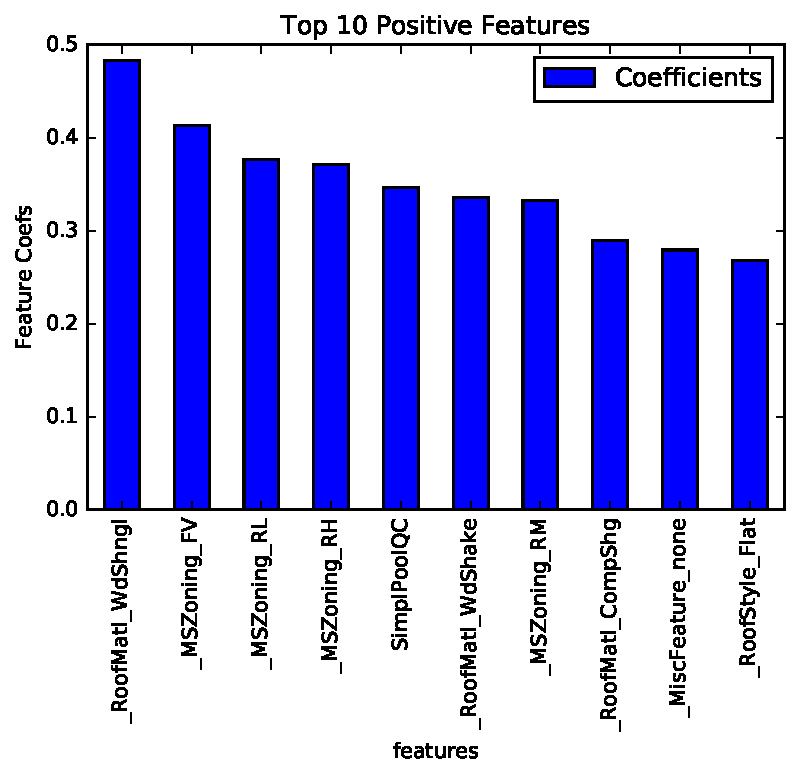
\includegraphics[width=0.8\columnwidth]{images/ridge_feature_ranking_pos}	
		\caption{Ridge Algorithm - Top 10 Positive Features} \label{fig:ridge_feature_ranking_pos} 
	\end{figure}
	
	\begin{figure}[H]
		\centering
		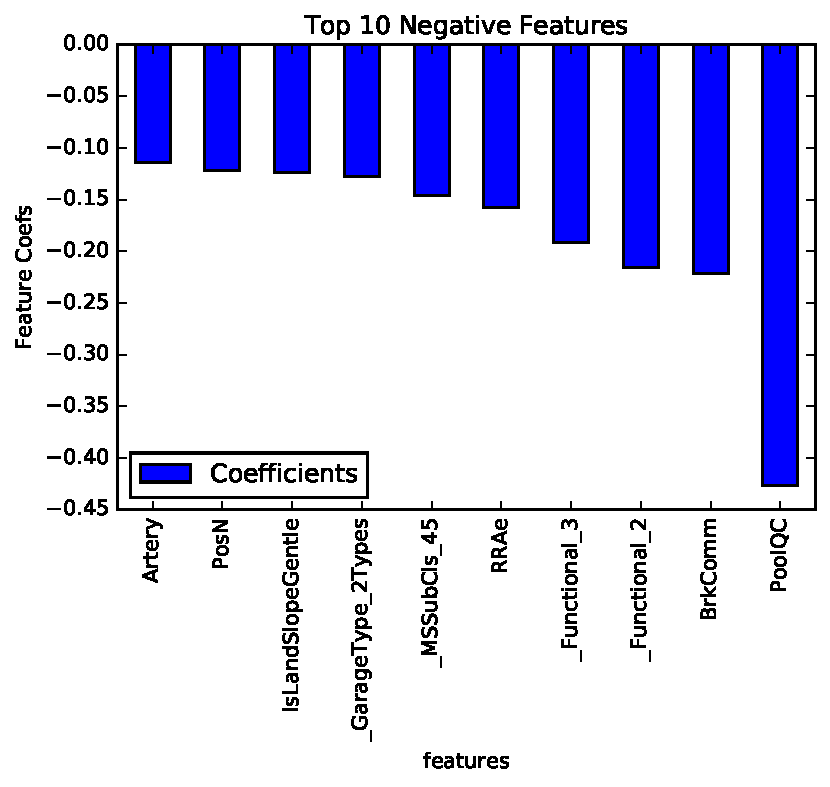
\includegraphics[width=0.8\columnwidth]{images/ridge_feature_ranking_neg}	
		\caption{Ridge Algorithm - Top 10 Negative Features} \label{fig:ridge_feature_ranking_neg} 
	\end{figure}
	
	\subsection{XGB Boosting Algorithm}
	
	XGBoost (eXtreme Gradient Boosting) is one of the Gradient Boosted Machine algorithms. It ensembles (combines) optimized model by taking trained models from all the preceding iterations. XGBoost regularizes the variables (parameters) to reduce the overfit and can work well with variables having missing values. It is empowered with built-in cross validation to reduce the boosting iterations; hence offers better performance along with parallel processing on distributed systems such as Hadoop. By tuning the XGBoost hyper parameters, we can achieve well optimized model that can make more accurate predictions. XGBoost uses {\em Fscore} to measure the importance of  variables. Following table explains the hyper-parameters of XGBoost algorithm and also given the python code implementing XGBoost algorithm for {\em sale price} predictions.
	
	\begin{table}[H]
		\center
		\caption{XGBoost Hyper-parameters}
		\label{tab:xgb_param}		
		\begin{tabular}{l p{5cm}}
			\toprule
			Hyper-parameter & Description \\
			\midrule
			Maximum Iterations: & Number of trees in the final model. More the trees, more accuracy. \\
			
			Maximum Depth: & Depth of each individual tree to control overfitting. \\
			
			Step Size: & Shrinkage, works similar to learning rate; smaller value takes more iterations. \\
			
			Column Subsample: & Subset of the columns to use in each iteratio.n \\ 
			\bottomrule
		\end{tabular}
	\end{table}
	
	\begin{verbatim}
	# python code - XGBoost algorithm
	import xgboost as xgb
	from xgboost import XGBClassifier
	from xgboost import plot_importance
	from sklearn.metrics import mean_squared_error
	from sklearn import cross_validation, metrics
	
	train = pd.read_csv("train.csv")
	test = pd.read_csv("test.csv")
	target_vector = train["SalePrice"]
	
	_algo = np.random.seed(1234)
	
	_xgb_algo = xgb.XGBRegressor(
	colsample_bytree=0.8,
	colsample_bylevel = 0.8,
	gamma=0.01,
	learning_rate=0.05,
	max_depth=5,
	min_child_weight=1.5,
	n_estimators=6000,                                                                  
	reg_alpha=0.5,
	reg_lambda=0.5,
	subsample=0.7,
	seed=42,
	silent=1)
	
	_xgb_algo.fit(train, target_vector)   
	
	feat_imp = pd.Series(_xgb_algo.booster()
	.get_fscore())
	.sort_values(ascending=False)[0:10] 
	plot = feat_imp.plot(kind='bar', 
	title='Top 10 Feature Importances')
	
	y_train = target_vector
	y_train_pred = _xgb_algo.predict(train)
	
	#root mean squared error (RMSE)
	rmse_train = np.sqrt(rmse(y_train,y_train_pred))
	
	y_test_pred = _xgb_algo.predict(test)
	
	\end{verbatim}
	
	
	\begin{figure}[H]
		\centering
		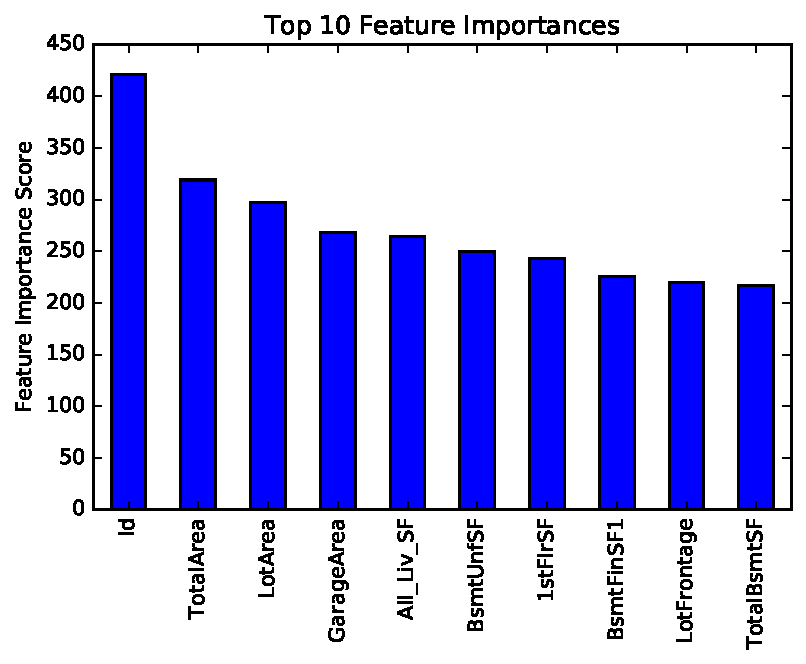
\includegraphics[width=0.75\columnwidth]{images/xgboost_feature_importance}	
		\caption{XGBoost Feature Importance} \label{fig:xgb_feature_imp} 
	\end{figure}
	
	
	\subsection{Neural Network Algorithm}
	
	\subsection{Model Ensembling}
	We can create a robust predictive model with better accuracy by merging two or more machine learning algorithms. This technique is called {\em model ensembling}. Ensembled algorithms may be similar in functionality or may entirely be different from each other. Individual algorithms may not perform great but by ensembling them, the overall system can offer much better performance and accuracy. Variations in the predicting logic in each of these individual algorithms will bring unbiasedness into the unified model. {\em Bagging}, {\em boosting} and {\em stacking} are popular ensembling techniques. Many of the advanced machine learning algorithms use ensembled approaches to achieve accurate classifications or predictions. Random Forest uses bagging, XGBoost uses boosting and Neural Network applies stacking ensembling techniques. For the kaggle submission, we have created an ensembled model by averaging {\em Sale Price} of the top 3 performing ensembled algorithms - XGBoost, Lasso and Neural Network.  Following are the kaggle public scores that we have achieved by submitting all the six algorithms along with the ensembled model. As predicted, ensembled model has scored better compared to the individual algorithms. By applying advanced machine learning algorithms, we have placed our scores within top 15\% of the competition. Following table displays each algorithm and the {\em root-mean-square error} (RMSE) along with the {\em kaggle score}.
	
	\begin{table}[H]
		\caption{Kaggle Submissions}
		\label{tab:kaggle}		
		\begin{tabular}{lrr}
			\toprule
			Algorithm & RMSE & Kaggle Score \\
			\midrule
			SVM &  0.2069 & 0.23967 \\
			Random Forest &  0.0519 & 0.14607 \\
			Ridge &  0.0988 & 0.13687 \\
			XGBoost &  0.0432 & 0.13018 \\					
			Lasso &  0.1015 & 0.12860 \\
			Neural Network &  0.20 & 0.12510 \\
			Ensemble &   & 0.12011 \\
			\bottomrule
		\end{tabular}
	\end{table}
	
	\section{Development Environment}
	
	\begin{itemize}
		\item Operating Environment: Ubuntu 16.4 through Oracle Virtual Box 5.2
		\item Programming Language: Python 2.7
		\item Development Tools/Environment: Jupyter Notebook, Anaconda (data science platform)
		\item Python Libraries: numpy, pandas, sklearn, matplotlib, seaborn, xgboost and tensorflow
		\item Repository: git@github.com:bigdata-i523/hid306.git
		\item Project Folders:
		\begin{itemize}
			\item Code: all Jupyter notebook files
			\item Images: all output images as PDF files
			\item Data: all the input and output datasets in CSV format
		\end{itemize}
		\item Python Jupyter notebook files:
		\begin{itemize}
			\item 1.1\_exploratory\_analysis\_numerical.ipynb
			\item 1.2\_exploratory\_analysis\_categorical.ipynb
			\item 1.3\_outlier\_and\_skewed\_data\_analysis.ipynb
			\item 1.4\_feature\_engineering.ipynb
			\item 2.1\_algorithm\_svm.ipynb
			\item 2.2\_algorithm\_random\_forest.ipynb
			\item 2.3\_algorithm\_ridge.ipynb
			\item 2.4\_algorithm\_lasso.ipynb
			\item 2.5\_algorithm\_neural\_network\_tf.ipynb
			\item 2.6\_algorithm\_xgboost.ipynb
			\item 3\_ensemble\_kaggle\_submission.ipynb	    	
		\end{itemize}
		\item Input Datasets: 
		\begin{itemize}
			\item train.csv
			\item test.csv
		\end{itemize}  
		\item Kaggle Submissions:
		\begin{itemize}
			\item kaggle\_python\_svm.csv
			\item kaggle\_python\_random\_forest.csv
			\item kaggle\_python\_ridge.csv
			\item kaggle\_python\_xgboost.csv
			\item kaggle\_python\_lasso.csv
			\item kaggle\_python\_neural\_network.csv
			\item kaggle\_python\_ensemble.csv
		\end{itemize}    	
	\end{itemize}    
	
	
	\section{Conclusion}
	
	Generally, ensemble models performs better compared to individual algorithms. However, there are a few factors that influence accuracy and performance of the algorithms, such as handcrafted feature engineering, proper cost function with regularized input to address non-linearities in the training datasets and tuning hyper-parameters of the algorithms. While Deep Learning Neural Networks are good for image processing, K-Nearest Neighbor algorithms can handle unsupervised datasets with less complexity. Domain knowledge and algorithm selection play vital role in getting accurate predictions. XGBoost, Random Forest, Lasso and Neural Networks are advanced machine learning algorithms dominating in the data science competitions for classification and regression related tasks. With ensembling and iterative learning techniques, they can scale well and offer better predictions for huge datasets having large number of features. 
	
	\appendix
	
	%Appendix A
	\section{Kaggle Housing Price Dataset Variables}
	
	\begin{itemize}
		\item Id: Row id
		\item SalePrice: Sale price of the house in dollars. This is the target variable to predict.
		\item MSSubClass: The building class
		\item MSZoning: The general zoning classification
		\item LotFrontage: Linear feet of street connected to property
		\item LotArea: Lot size in square feet
		\item Street: Type of road access
		\item Alley: Type of alley access
		\item LotShape: General shape of property
		\item LandContour: Flatness of the property
		\item Utilities: Type of utilities available
		\item LotConfig: Lot configuration
		\item LandSlope: Slope of property
		\item Neighborhood: Physical locations within Ames city limits
		\item Condition1: Proximity to main road or railroad
		\item Condition2: Proximity to main road or railroad (if a second is present)
		\item BldgType: Type of dwelling
		\item HouseStyle: Style of dwelling
		\item OverallQual: Overall material and finish quality
		\item OverallCond: Overall condition rating
		\item YearBuilt: Original construction date
		\item YearRemodAdd: Remodel date
		\item RoofStyle: Type of roof
		\item RoofMatl: Roof material
		\item Exterior1st: Exterior covering on house
		\item Exterior2nd: Exterior covering on house (if more than one material)
		\item MasVnrType: Masonry veneer type
		\item MasVnrArea: Masonry veneer area in square feet
		\item ExterQual: Exterior material quality
		\item ExterCond: Present condition of the material on the exterior
		\item Foundation: Type of foundation
		\item BsmtQual: Height of the basement
		\item BsmtCond: General condition of the basement
		\item BsmtExposure: Walkout or garden level basement walls
		\item BsmtFinType1: Quality of basement finished area
		\item BsmtFinSF1: Type 1 finished square feet
		\item BsmtFinType2: Quality of second finished area (if present)
		\item BsmtFinSF2: Type 2 finished square feet
		\item BsmtUnfSF: Unfinished square feet of basement area
		\item TotalBsmtSF: Total square feet of basement area
		\item Heating: Type of heating
		\item HeatingQC: Heating quality and condition
		\item CentralAir: Central air conditioning Electrical: Electrical system
		\item 1stFlrSF: First Floor square feet
		\item 2ndFlrSF: Second floor square feet
		\item LowQualFinSF: Low quality finished square feet (all floors)
		\item GrLivArea: Above grade (ground) living area square feet
		\item BsmtFullBath: Basement full bathrooms
		\item BsmtHalfBath: Basement half bathrooms
		\item FullBath: Full bathrooms above grade
		\item HalfBath: Half baths above grade
		\item Bedroom: Number of bedrooms above basement level
		\item Kitchen: Number of kitchens
		\item KitchenQual: Kitchen quality
		\item TotRmsAbvGrd: Total rooms above grade (does not include bathrooms)
		\item Functional: Home functionality rating
		\item Fireplaces: Number of fireplaces
		\item FireplaceQu: Fireplace quality
		\item GarageType: Garage location
		\item GarageYrBlt: Year garage was built
		\item GarageFinish: Interior finish of the garage
		\item GarageCars: Size of garage in car capacity
		\item GarageArea: Size of garage in square feet
		\item GarageQual: Garage quality
		\item GarageCond: Garage condition
		\item PavedDrive: Paved driveway
		\item WoodDeckSF: Wood deck area in square feet
		\item OpenPorchSF: Open porch area in square feet
		\item EnclosedPorch: Enclosed porch area in square feet
		\item 3SsnPorch: Three season porch area in square feet
		\item ScreenPorch: Screen porch area in square feet
		\item PoolArea: Pool area in square feet
		\item PoolQC: Pool quality
		\item Fence: Fence quality
		\item MiscFeature: Miscellaneous feature not covered in other categories
		\item MiscVal: Dollar Value of miscellaneous feature
		\item MoSold: Month Sold
		\item YrSold: Year Sold
		\item SaleType: Type of sale
		\item SaleCondition: Condition of sale
	\end{itemize}
	
	\nocite{*}
	
	\begin{acks}	
		The authors would like to thank Dr. Gregor von Laszewski and the Teaching Assistants for their support and great suggestions. Authors would also want to thank Kaggle Website and the developers for their valuable information, ideas and contributions.		
	\end{acks}
	
	
	\bibliographystyle{ACM-Reference-Format}
	\bibliography{report} 	
	
	
\end{document}
